\notechapter{N-20240427}{Differential Forms and Stokes: Measuring, Pulling Back, and Integrating Geometry}

\section{Why forms are not just notation}

Expressions such as \(dx\), \(dy\), and \(dx\wedge dy\) can look like formal decorations. Differential forms give them a precise meaning. They are the objects that can be pulled back and integrated in a coordinate-compatible way.

A differential form is a geometric measuring device. A \(1\)-form measures tangent vectors. A \(2\)-form measures oriented parallelograms. A \(k\)-form measures oriented \(k\)-dimensional infinitesimal volume.

\section{Covectors and one-forms}

At a point \(p\), a tangent vector lives in \(T_pM\). A covector is a linear functional
\[
  \alpha:T_pM\to\mathbb R.
\]
The space of covectors is the dual space \(T_p^*M\).

In coordinates, a \(1\)-form looks like
\[
  \omega=P(x,y)\,dx+Q(x,y)\,dy.
\]
If \(v=a\frac{\partial}{\partial x}+b\frac{\partial}{\partial y}\), then
\[
  \omega(v)=Pa+Qb.
\]
So a \(1\)-form is not a tiny vector. It is a rule for measuring vectors.

\section{Wedge products}

The wedge product is alternating:
\[
  dx\wedge dy=-dy\wedge dx,\qquad dx\wedge dx=0.
\]
This sign is the algebraic memory of orientation. Reversing the order of two directions reverses the sign of an oriented area.

A typical \(2\)-form in the plane is
\[
  f(x,y)\,dx\wedge dy.
\]
It measures signed area with density \(f\).

\section{Exterior derivative}

The exterior derivative turns \(k\)-forms into \((k+1)\)-forms. For a function \(f\),
\[
  df=\frac{\partial f}{\partial x}\,dx+\frac{\partial f}{\partial y}\,dy.
\]
For a \(1\)-form \(\omega=P\,dx+Q\,dy\),
\[
  d\omega=\left(\frac{\partial Q}{\partial x}-\frac{\partial P}{\partial y}\right)dx\wedge dy.
\]
The universal rule is
\[
  d^2=0.
\]
This single formula contains familiar facts such as curl of gradient equals zero and divergence of curl equals zero.

\section{Closed and exact}

A form \(\omega\) is closed if \(d\omega=0\). It is exact if there exists a form \(\eta\) such that
\[
  \omega=d\eta.
\]
Exact forms are always closed because \(d^2=0\). The converse is local but not always global. This is one of the first hints that differential forms remember topology.

\section{Pullbacks}

If \(F:N\to M\) is smooth and \(\omega\) is a form on \(M\), the pullback \(F^*\omega\) is a form on \(N\). It tells us how to measure on \(N\) using a form originally defined on \(M\).

For a function \(f\), \(F^*f=f\circ F\). For differentials,
\[
  F^*(df)=d(F^*f).
\]
This is the cleanest conceptual form of the chain rule.

\section{Integration needs orientation}

To integrate a form, we need an oriented domain. Orientation decides which order of basis vectors counts as positive. Without orientation, \(dx\wedge dy\) has no consistent sign.

The boundary of an oriented region also receives an orientation. This sign bookkeeping is not cosmetic; it is exactly what makes Stokes' theorem true.

\begin{figure}[H]
\centering
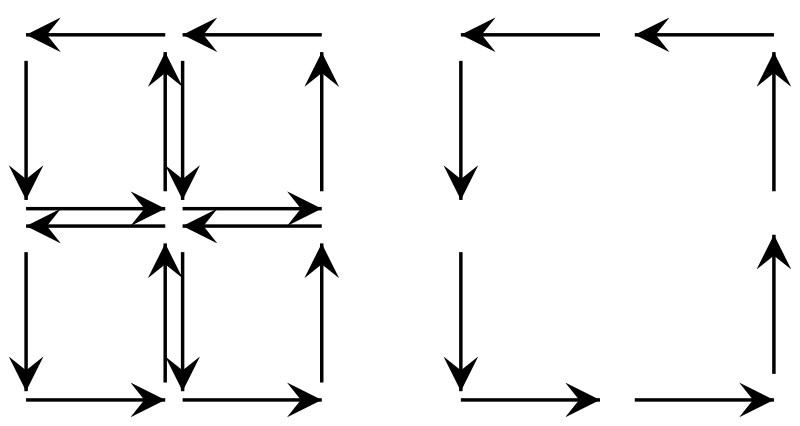
\includegraphics[width=.55\linewidth]{figures/N-20240427/stokes-patch.png}
\caption{A small oriented patch: the boundary orientation is part of the theorem.}
\end{figure}

\section{Stokes' theorem}

The central theorem is
\[
  \int_M d\omega=\int_{\partial M}\omega.
\]
This is Stokes' theorem. It says that the integral of a derivative over a region is controlled by the original quantity on the boundary.

Many familiar theorems are shadows of this one:
\[
\begin{array}{c|c}
\text{classical theorem} & \text{form-theoretic statement}\\
\hline
\text{Fundamental theorem of calculus} & \int_{[a,b]}df=f(b)-f(a)\\
\text{Green's theorem} & \int_D d(P\,dx+Q\,dy)=\int_{\partial D}P\,dx+Q\,dy\\
\text{Divergence theorem} & \int_M d\omega=\int_{\partial M}\omega
\end{array}
\]


% line integrals expanded example
\section{A worked example: line integrals}

Let
\[
  \omega=P(x,y)\,dx+Q(x,y)\,dy
\]
and let \(\gamma(t)=(x(t),y(t))\), \(a\le t\le b\). Pulling back \(\omega\) to the interval gives
\[
  \gamma^*\omega=\left(P(x(t),y(t))x'(t)+Q(x(t),y(t))y'(t)\right)dt.
\]
Thus
\[
  \int_\gamma \omega
  =\int_a^b
  \left(P(x(t),y(t))x'(t)+Q(x(t),y(t))y'(t)\right)dt.
\]
This is the usual line integral, but now it is explained by one operation: pull back the form to the parameter domain and integrate there.

\section{A worked example: Green's theorem}

For \(\omega=P\,dx+Q\,dy\),
\[
  d\omega=\left(\frac{\partial Q}{\partial x}-\frac{\partial P}{\partial y}\right)dx\wedge dy.
\]
Stokes' theorem on a planar region \(D\) says
\[
  \int_D d\omega=\int_{\partial D}\omega.
\]
In coordinates this becomes
\[
  \iint_D\left(\frac{\partial Q}{\partial x}-\frac{\partial P}{\partial y}\right)dx\,dy
  =\int_{\partial D}P\,dx+Q\,dy.
\]
So Green's theorem is not a separate miracle. It is Stokes' theorem written in two-dimensional coordinates.

\section{Why arc length is different}

A common confusion is to treat \(ds\) like a \(1\)-form. But arc length is not linear in the velocity:
\[
  ds(\gamma')=\|\gamma'\|dt.
\]
The norm is not a linear functional. Differential forms measure oriented quantities; metrics measure lengths and angles. Both are geometric, but they are not the same kind of structure.

\section{Why this viewpoint is worth learning}

Vector calculus has several different-looking integral theorems. Differential forms reveal one pattern behind them. Derivatives become exterior derivatives. Change of variables becomes pullback. Boundary signs become orientation. Integrals become pairings of forms with domains.

The slogan is:
\[
  \text{Stokes says that local change becomes boundary measurement.}
\]
